\documentclass{standalone}

%----------------------------------------------------------------------------------------------%
%                                 Packages and basic declarations
%----------------------------------------------------------------------------------------------%

\usepackage{amsmath}
\usepackage{mathrsfs}
\usepackage{pgf}
\usepackage{tikz}
\usepackage{verbatim}


\usetikzlibrary{arrows}


\tikzset{
  font={\fontsize{36pt}{32}\selectfont}}

%----------------------------------------------------------------------------------------------%
%----------------------------------------------------------------------------------------------%
%                                            DOCUMENT STARTS
%----------------------------------------------------------------------------------------------%
%----------------------------------------------------------------------------------------------%

\begin{document}

%----------------------------------------------------------------------------------------------%
%                Single RVE with applied constant strain, only debonded
%----------------------------------------------------------------------------------------------%

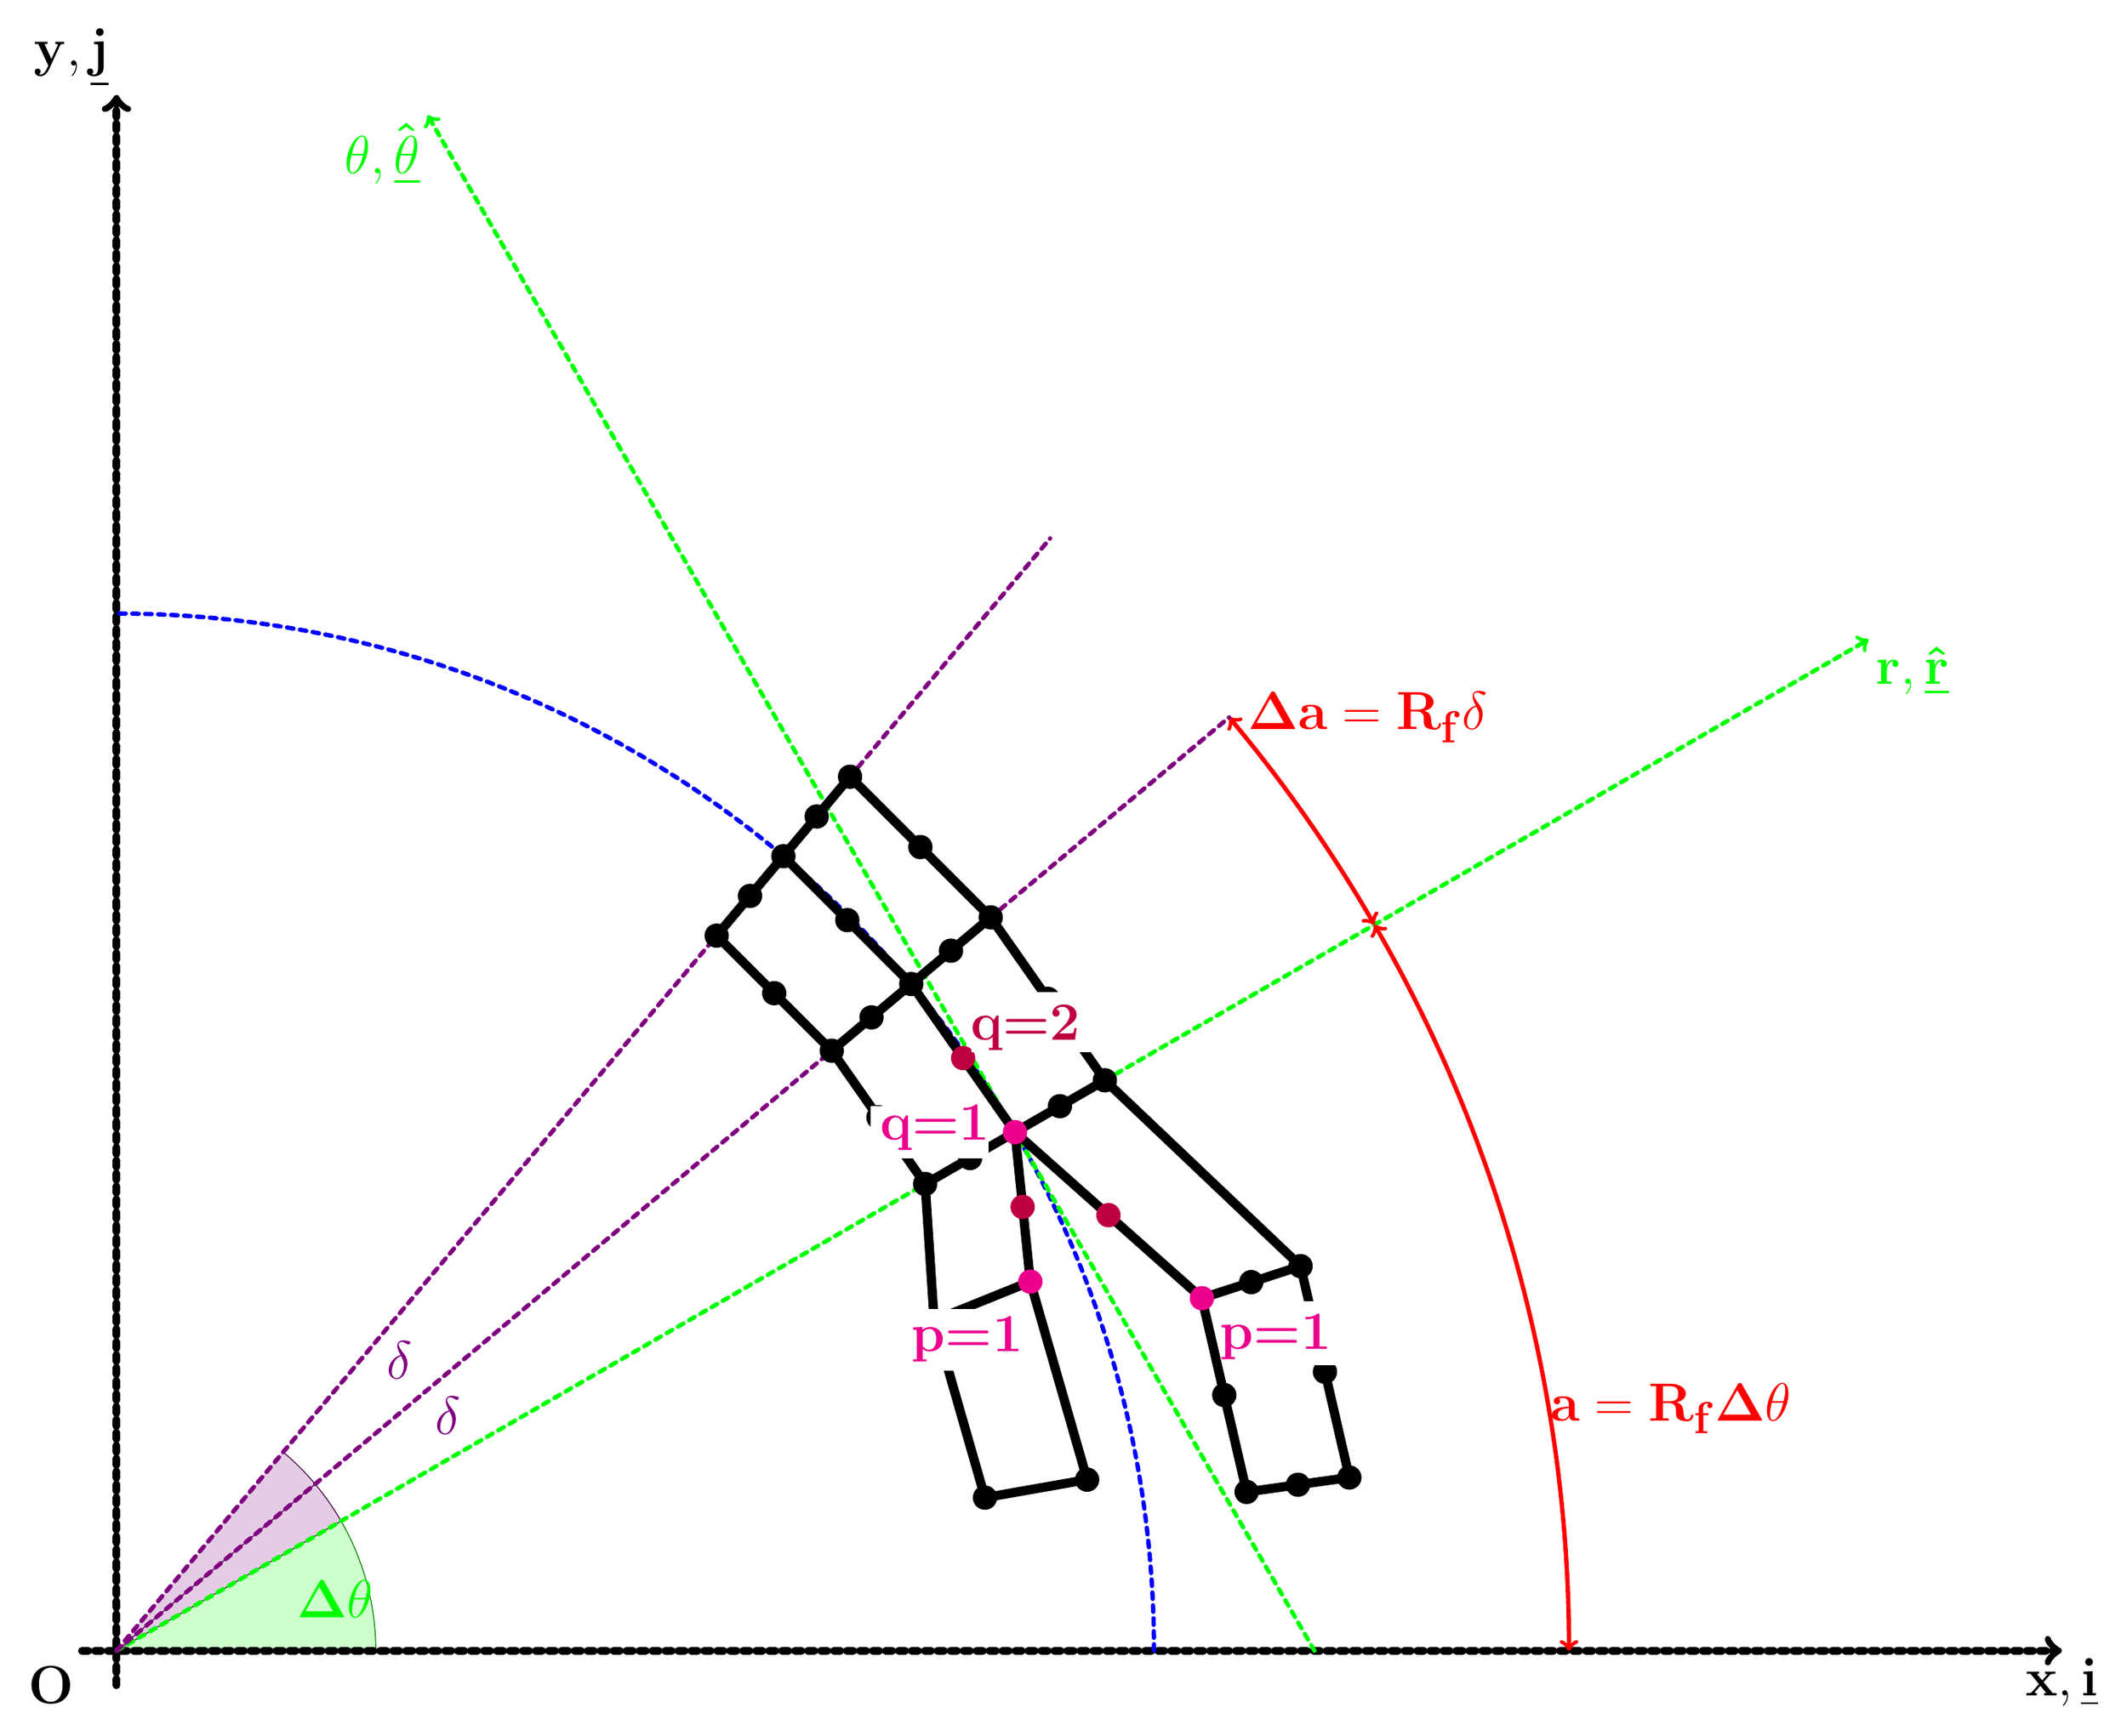
\begin{tikzpicture}[scale=7.5,cap=round,x=1.5cm,y=1.5cm]

%----------------------------------------------------------------------------------------------%
%                                                   CONSTANTS
%----------------------------------------------------------------------------------------------%

\def\pivalue{3.141592653589793238462643383279502884197169399375105820974944592307816406286}

\def\R{1.5}
\pgfmathsetmacro\lim{1.5*\R}
\def\xC{0.0}
\def\yC{0.0}

\pgfmathsetmacro\xCT{\R*cos(30)}
\pgfmathsetmacro\yCT{\R*sin(30)}
\pgfmathsetmacro\xBO{0.5*\R*(cos(30)+cos(40))}
\pgfmathsetmacro\yBO{0.5*\R*(sin(30)+sin(40))}
\pgfmathsetmacro\xA{\R*cos(40)}
\pgfmathsetmacro\yA{\R*sin(40)}
\pgfmathsetmacro\xB{\R*cos(50)}
\pgfmathsetmacro\yB{\R*sin(50)}
\pgfmathsetmacro\xC{0.95*\R*cos(22)}
\pgfmathsetmacro\yC{0.95*\R*sin(22)}
\pgfmathsetmacro\xCC{0.5*\R*(0.95*cos(22)+cos(30))}
\pgfmathsetmacro\yCC{0.5*\R*(0.95*sin(22)+sin(30))}
\pgfmathsetmacro\xD{0.95*\R*cos(10)}
\pgfmathsetmacro\yD{0.95*\R*sin(10)}
\pgfmathsetmacro\xE{1.10*\R*cos(18)}
\pgfmathsetmacro\yE{1.10*\R*sin(18)}
\pgfmathsetmacro\xEE{0.5*\R*(1.1*cos(18)+cos(30))}
\pgfmathsetmacro\yEE{0.5*\R*(1.1*sin(18)+sin(30))}
\pgfmathsetmacro\xF{1.10*\R*cos(8)}
\pgfmathsetmacro\yF{1.10*\R*sin(8)}

\pgfmathsetmacro\xCTBF{0.9*\R*cos(30)}
\pgfmathsetmacro\yCTBF{0.9*\R*sin(30)}
\pgfmathsetmacro\xABF{0.9*\R*cos(40)}
\pgfmathsetmacro\yABF{0.9*\R*sin(40)}
\pgfmathsetmacro\xBBF{0.9*\R*cos(50)}
\pgfmathsetmacro\yBBF{0.9*\R*sin(50)}
\pgfmathsetmacro\xCBF{0.85*\R*cos(22)}
\pgfmathsetmacro\yCBF{0.85*\R*sin(22)}
\pgfmathsetmacro\xDBF{0.85*\R*cos(10)}
\pgfmathsetmacro\yDBF{0.85*\R*sin(10)}

\pgfmathsetmacro\xCTBM{1.1*\R*cos(30)}
\pgfmathsetmacro\yCTBM{1.1*\R*sin(30)}
\pgfmathsetmacro\xABM{1.1*\R*cos(40)}
\pgfmathsetmacro\yABM{1.1*\R*sin(40)}
\pgfmathsetmacro\xBBM{1.1*\R*cos(50)}
\pgfmathsetmacro\yBBM{1.1*\R*sin(50)}
\pgfmathsetmacro\xEBM{1.20*\R*cos(18)}
\pgfmathsetmacro\yEBM{1.20*\R*sin(18)}
\pgfmathsetmacro\xFBM{1.20*\R*cos(8)}
\pgfmathsetmacro\yFBM{1.20*\R*sin(8)}

\pgfmathsetmacro\xG{1.4*\R*cos(30)}
\pgfmathsetmacro\yG{1.4*\R*sin(30)}

\pgfmathsetmacro\xH{1.4*\R*cos(40)}
\pgfmathsetmacro\yH{1.4*\R*sin(40)}

\pgfmathsetmacro\xHH{1.4*\R*cos(50)}
\pgfmathsetmacro\yHH{1.4*\R*sin(50)}

\pgfmathsetmacro\xI{0.25*\R*cos(30)}
\pgfmathsetmacro\yI{0.25*\R*sin(30)}

\pgfmathsetmacro\xII{0.25*\R*cos(40)}
\pgfmathsetmacro\yII{0.25*\R*sin(40)}

\pgfmathsetmacro\xAtoB{0.5*(\xA+\xB)}
\pgfmathsetmacro\yAtoB{0.5*(\yA+\yB)}
\pgfmathsetmacro\xEtoF{0.5*(\xE+\xF)}
\pgfmathsetmacro\yEtoF{0.5*(\yE+\yF)}
\pgfmathsetmacro\xBtoBBF{0.5*(\xB+\xBBF)}
\pgfmathsetmacro\yBtoBBF{0.5*(\yB+\yBBF)}
\pgfmathsetmacro\xBtoBBM{0.5*(\xB+\xBBM)}
\pgfmathsetmacro\yBtoBBM{0.5*(\yB+\yBBM)}
\pgfmathsetmacro\xAtoABF{0.5*(\xA+\xABF)}
\pgfmathsetmacro\yAtoABF{0.5*(\yA+\yABF)}
\pgfmathsetmacro\xAtoABM{0.5*(\xA+\xABM)}
\pgfmathsetmacro\yAtoABM{0.5*(\yA+\yABM)}
\pgfmathsetmacro\xCTtoCTBF{0.5*(\xCT+\xCTBF)}
\pgfmathsetmacro\yCTtoCTBF{0.5*(\yCT+\yCTBF)}
\pgfmathsetmacro\xCTtoCTBM{0.5*(\xCT+\xCTBM)}
\pgfmathsetmacro\yCTtoCTBM{0.5*(\yCT+\yCTBM)}
\pgfmathsetmacro\xEtoEBM{0.5*(\xE+\xEBM)}
\pgfmathsetmacro\yEtoEBM{0.5*(\yE+\yEBM)}
\pgfmathsetmacro\xFtoFBM{0.5*(\xF+\xFBM)}
\pgfmathsetmacro\yFtoFBM{0.5*(\yF+\yFBM)}
\pgfmathsetmacro\xBBFtoABF{0.5*(\xBBF+\xABF)}
\pgfmathsetmacro\yBBFtoABF{0.5*(\yBBF+\yABF)}
\pgfmathsetmacro\xBBMtoABM{0.5*(\xBBM+\xABM)}
\pgfmathsetmacro\yBBMtoABM{0.5*(\yBBM+\yABM)}
\pgfmathsetmacro\xCTBFtoABF{0.5*(\xCTBF+\xABF)}
\pgfmathsetmacro\yCTBFtoABF{0.5*(\yCTBF+\yABF)}
\pgfmathsetmacro\xCTBMtoABM{0.5*(\xCTBM+\xABM)}
\pgfmathsetmacro\yCTBMtoABM{0.5*(\yCTBM+\yABM)}
\pgfmathsetmacro\xEBMtoFBM{0.5*(\xEBM+\xFBM)}
\pgfmathsetmacro\yEBMtoFBM{0.5*(\yEBM+\yFBM)}

\def\xFin{0.45}
\pgfmathsetmacro\yFin{-sqrt(3)*\xFin+(\yCT+sqrt(3)*\xCT)}
\pgfmathsetmacro\xIntersect{(\yCT+sqrt(3)*\xCT)/sqrt(3)}

\filldraw[fill=green!20,draw=green!50!black] (0,0) -- (0.25*\R,0) arc(0:30:0.25*\R);
\filldraw[fill=violet!20,draw=violet!50!black] (0,0) -- (\xI,\yI) arc(30:40:0.25*\R);
\filldraw[fill=violet!20,draw=violet!50!black] (0,0) -- (\xII,\yII) arc(40:50:0.25*\R);

\draw[->,dashed, line width = 1.25mm] (-0.05,0.0) -- (1.25*\lim,0.0);
\node[anchor=north] at (1.25*\lim,0.0) {\Huge $\mathbf{x,\underline{i}}$};
\draw[->,dashed, line width = 1.25mm] (0.0,-0.05)  -- (0.0,\lim) ;
\node[anchor=south east] at (0.0,\lim) {\Huge $\mathbf{y,\underline{j}}$};

\node[text=black,anchor=east] at (-0.05,-0.05) {\Huge $\mathbf{O}$};

\draw[draw=blue,dashed,line width=2pt](\R,0) arc(0:90:\R);
\draw[->,draw=green,dashed,line width=2pt] (0,0)  -- (1.95*\xCT,1.95*\yCT) ;
\draw[->,draw=green,dashed,line width=2pt] (\xIntersect,0)  -- (\xFin,\yFin) ;

\draw[<->,draw=red,line width=2pt](1.4*\R,0) arc(0:30:1.4*\R);
\draw[<->,draw=red,line width=2pt](\xG,\yG) arc(30:40:1.4*\R);

\draw[draw=violet,dashed,line width=2pt] (0,0)  -- (\xH,\yH) ;
\draw[draw=violet,dashed,line width=2pt] (0,0)  -- (\xHH,\yHH) ;

\draw[line width=1.5mm] (\xB,\yB) -- (\xA,\yA) -- (\xCT,\yCT)  -- (\xC,\yC)  -- (\xD,\yD) ;
\draw[line width=1.5mm] (\xCT,\yCT)  -- (\xE,\yE)  -- (\xF,\yF) ;
\draw[line width=1.5mm] (\xBBF,\yBBF) -- (\xABF,\yABF) -- (\xCTBF,\yCTBF)  -- (\xCBF,\yCBF)  -- (\xDBF,\yDBF) ;
\draw[line width=1.5mm] (\xBBM,\yBBM) -- (\xABM,\yABM) -- (\xCTBM,\yCTBM)  -- (\xEBM,\yEBM)  -- (\xFBM,\yFBM) ;
\draw[line width=1.5mm] (\xBBM,\yBBM) -- (\xB,\yB) -- (\xBBF,\yBBF) ;
\draw[line width=1.5mm] (\xABM,\yABM) -- (\xA,\yA) -- (\xABF,\yABF) ;
\draw[line width=1.5mm] (\xCTBM,\yCTBM) -- (\xCT,\yCT) -- (\xCTBF,\yCTBF) ;
\draw[line width=1.5mm] (\xDBF,\yDBF) -- (\xD,\yD);
\draw[line width=1.5mm] (\xCBF,\yCBF) -- (\xC,\yC);
\draw[line width=1.5mm] (\xEBM,\yEBM) -- (\xE,\yE);
\draw[line width=1.5mm] (\xFBM,\yFBM) -- (\xF,\yF);

\foreach \Point in {(\xB,\yB),(\xA,\yA),(\xD,\yD),(\xF,\yF)}{
    \fill \Point  circle[radius=0.75pt];
}
\foreach \Point in {(\xBBF,\yBBF),(\xABF,\yABF),(\xCTBF,\yCTBF),(\xCBF,\yCBF),(\xDBF,\yDBF)}{
    \fill \Point  circle[radius=0.75pt];
}
\foreach \Point in {(\xBBM,\yBBM),(\xABM,\yABM),(\xCTBM,\yCTBM),(\xEBM,\yEBM),(\xFBM,\yFBM)}{
    \fill \Point  circle[radius=0.75pt];
}

\foreach \Point in {(\xAtoB,\yAtoB),(\xBtoBBF,\yBtoBBF),(\xBtoBBM,\yBtoBBM),(\xAtoABF,\yAtoABF),(\xAtoABM,\yAtoABM),(\xCTtoCTBF,\yCTtoCTBF),(\xCTtoCTBM,\yCTtoCTBM),(\xEtoEBM,\yEtoEBM),(\xFtoFBM,\yFtoFBM),(\xBBMtoABM,\yBBMtoABM),(\xBBFtoABF,\yBBFtoABF),(\xCTBMtoABM,\yCTBMtoABM),(\xCTBFtoABF,\yCTBFtoABF),(\xEtoF,\yEtoF),(\xEBMtoFBM,\yEBMtoFBM)}{
    \fill \Point  circle[radius=0.75pt];
}

\fill[fill=magenta] (\xCT,\yCT)  circle[radius=0.75pt];
\fill[fill=purple] (\xBO,\yBO)  circle[radius=0.75pt];
\fill[fill=magenta] (\xC,\yC)  circle[radius=0.75pt];
\fill[fill=purple] (\xCC,\yCC)  circle[radius=0.75pt];
\fill[fill=magenta] (\xE,\yE)  circle[radius=0.75pt];
\fill[fill=purple] (\xEE,\yEE)  circle[radius=0.75pt];

\node[anchor= west,text=green] at (0.25,0.075) {\Huge $\mathbf{\Delta\theta}$};
\node[anchor= west,text=violet] at (0.45,0.34) {\Huge $\mathbf{\delta}$};
\node[anchor= west,text=violet] at (0.38,0.42) {\Huge $\mathbf{\delta}$};
\node[anchor= west,text=red] at (1.375*\R,0.35) {\Huge $\mathbf{a = R_{f}\Delta\theta}$};
\node[anchor= west,text=red] at (1.01*\xH,\yH) {\Huge $\mathbf{\Delta a = R_{f}\delta}$};
\node[anchor= north west,text=green] at (1.95*\xCT,1.95*\yCT)  {\Huge $\mathbf{r,\hat{\underline{r}}}$};
\node[anchor= north east,text=green] at (\xFin,\yFin)  {\Huge $\mathbf{\theta,\hat{\underline{\theta}}}$};
\draw[white,fill=white] (0.84*\xCT,0.95*\yCT) rectangle(0.97*\xCT,1.05*\yCT);
\node[anchor= south east,text=magenta] at (0.98*\xCT,0.95*\yCT)  {\Huge \bf{q=1}};
\draw[white,fill=white] (1.01*\xBO,1.01*\yBO) rectangle(1.15*\xBO,1.11*\yBO);
\node[anchor= south west,text=purple] at (\xBO,\yBO)  {\Huge \bf{q=2}};
\draw[white,fill=white] (0.85*\xC,0.76*\yC) rectangle(\xC,0.925*\yC);
\node[anchor= north east,text=magenta] at (\xC,0.925*\yC)  {\Huge \bf{p=1}};
\draw[white,fill=white] (1.02*\xE,0.81*\yE) rectangle(1.15*\xE,0.99*\yE);
\node[anchor= north west,text=magenta] at (1.01*\xE,0.975*\yE)  {\Huge \bf{p=1}};

\end{tikzpicture}

\end{document}
